\subsection{问题一：温度关系与时间变化}

本问分别处理附件1和附件2。对于附件1，本文用直线概括每种催化剂组合的平均温度
关系，并用相邻观测保留局部变化；对于附件2，本文按真实时间计算转化率、
选择性、收率和产物份额的变化。两部分均先给出计算关系，再报告结果和适用范围。

\subsubsection{附件 1：各催化剂组合的温度关系}

\paragraph{相邻温度下的实际变化}

对任一组合 \(i\)，将实际测试温度按
\(T_{i1}<T_{i2}<\cdots<T_{in_i}\) 排列。为保留已测条件之间的
真实变化，定义相邻温度指标差：

\begin{align}
\Delta X_{ij}&=X_i(T_{i,j+1})-X_i(T_{ij}), \tag{2}\label{eq:q1-adjacent-x}\\
\Delta S_{ij}&=S_i(T_{i,j+1})-S_i(T_{ij}). \tag{3}\label{eq:q1-adjacent-s}
\end{align}

当差值大于 0、等于 0 或小于 0 时，分别表示较高温度条件下指标上升、持平或局部
下降。式\eqref{eq:q1-adjacent-x}和式\eqref{eq:q1-adjacent-s}只连接附件中真实存在的相邻温度，不补造中间温度，也不把连线
解释为同一次连续升温过程。

各组合只使用自身实际存在的温度点，不补齐缺失温度。若全部相邻差值为正，则该指标在
已测相邻温度下均升高；若出现负值或零值，则记录相应温区和变化量。

以A5的转化率为例，250 ℃和275 ℃的观测值分别为14.7872\%和12.4240\%，所以该区间
转化率变化为：

\[
\Delta X_{\mathrm{A5}}=12.4240\%-14.7872\%=-2.3632\text{ 个百分点}.
\]

该负值直接说明A5在250---275 ℃之间出现局部下降。即使后续直线给出A5在全部已测范围
内的平均斜率为正，这一离散事实也必须保留。

图\ref{fig:q1-adjacent-map}汇总所有组合在相邻已测温度之间的实际变化。
\begin{figure}[H]
\centering
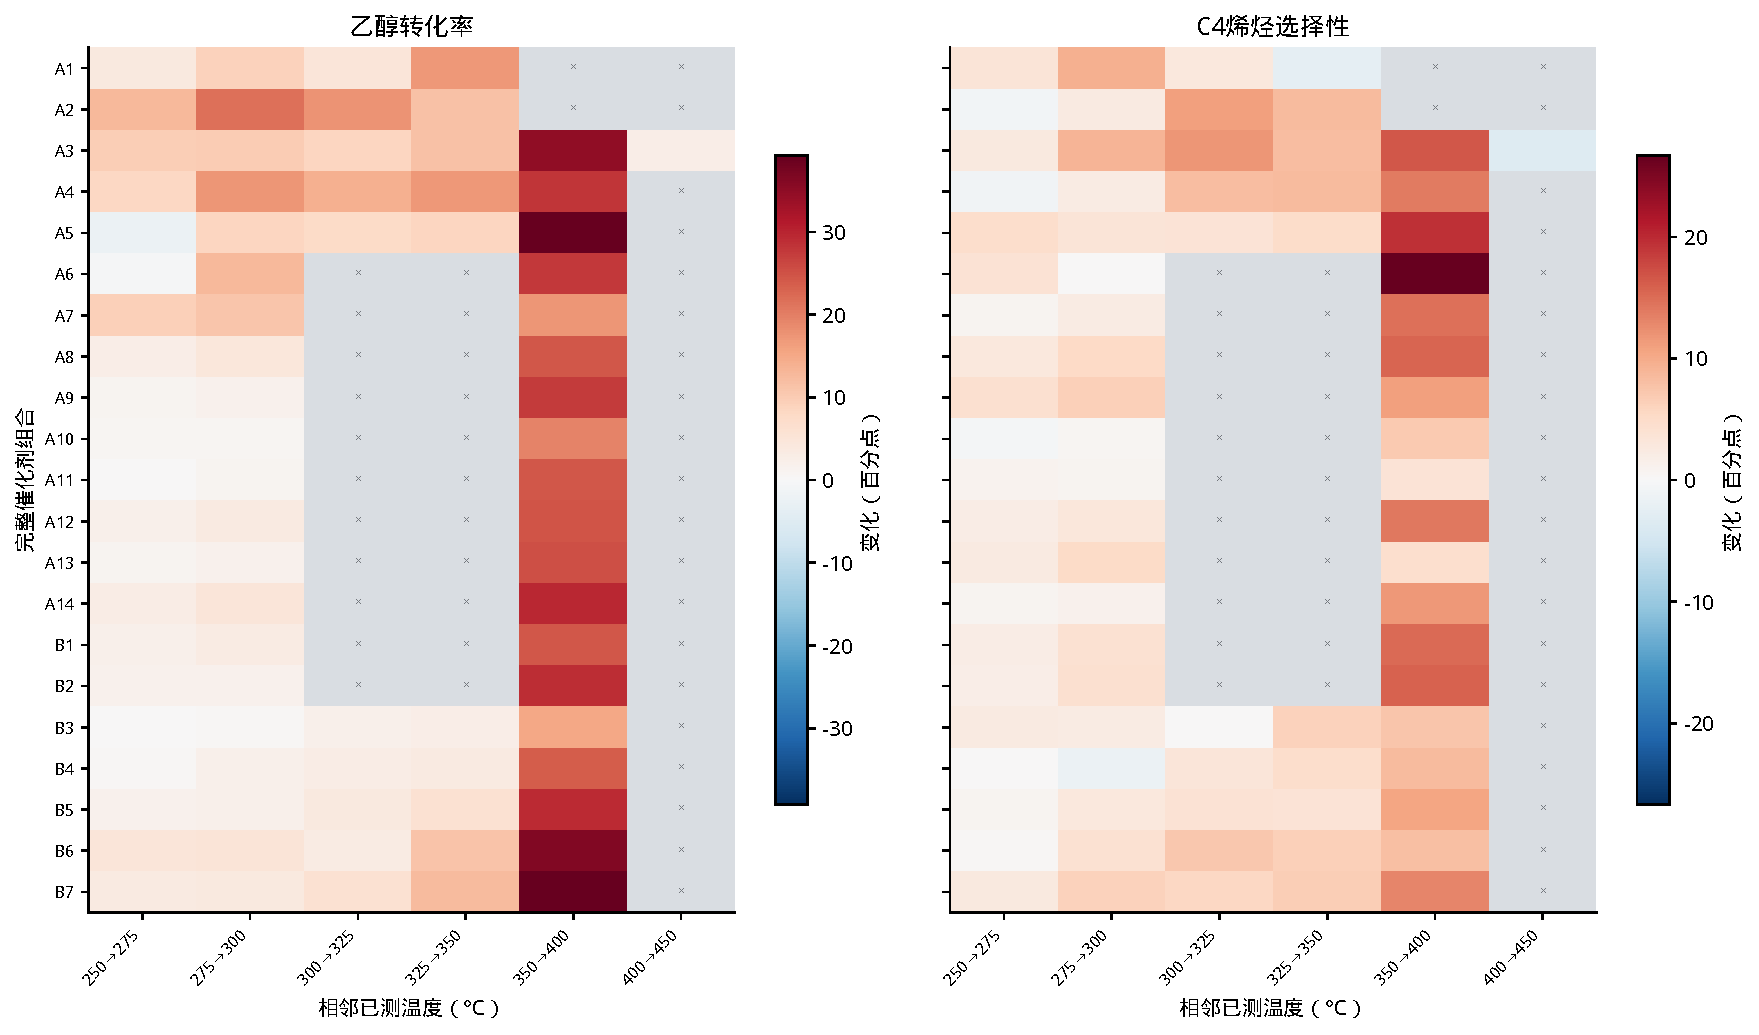
\includegraphics[width=0.82\linewidth]{../../output/q1/figures/02_adjacent_temperature_change_map.pdf}
\caption{各催化剂组合在相邻已测温度间的指标变化。暖色表示指标上升，冷色表示下降，
接近白色表示变化接近零，灰色叉号表示该组合不存在相应温度区间。}
\label{fig:q1-adjacent-map}
\end{figure}

暖色单元占多数，说明较高温度通常
对应较高的转化率和选择性；冷色或接近零的单元标出局部下降和持平。灰色叉号表示该
组合没有相应温区的记录。

\paragraph{每种组合的平均温度关系}

相邻差值能够显示局部变化，但不便于比较21种组合的平均升温幅度。因此，本文对每种
组合的转化率和选择性分别作一元最小二乘线性拟合：

\begin{align}
X_{ij}&=a_i^X+b_i^XT_{ij}+e_{ij}^X, \tag{4}\\
S_{ij}&=a_i^S+b_i^ST_{ij}+e_{ij}^S. \tag{5}
\end{align}

其中，$b_i^X$ 和 $b_i^S$ 分别表示温度每升高1 ℃时转化率和选择性的平均变化，
$e_{ij}$ 表示观测值与直线之间的差。为便于比较，结果统一报告 \(25b\)，即温度每升高
25 ℃时指标平均改变的百分点数。

对某一组合的某一个指标，统一记观测值为 $Z_{ij}$，样本均值为 $\bar T_i$ 和 $\bar Z_i$。使用最小二乘
法选择斜率，使全部观测点到直线的纵向偏差平方和最小。斜率和截距分别为：

\begin{align}
b_i&=\frac{\sum_j(T_{ij}-\bar T_i)(Z_{ij}-\bar Z_i)}
{\sum_j(T_{ij}-\bar T_i)^2}, \tag{6}\label{eq:q1-ols-slope}\\
a_i&=\bar Z_i-b_i\bar T_i. \tag{7}\label{eq:q1-ols-intercept}
\end{align}

将实际温度代入直线得到拟合值 \(\widehat Z_{ij}=a_i+b_iT_{ij}\)，残差为
\(e_{ij}=Z_{ij}-\widehat Z_{ij}\)。式\eqref{eq:q1-ols-slope}直接使用温度数值，因此能够处理不同的
温度间隔。

为说明直线对该组观测的概括程度，计算决定系数：

\begin{equation}
R_i^2=1-\frac{\sum_j e_{ij}^2}{\sum_j(Z_{ij}-\bar Z_i)^2}.
\tag{8}
\end{equation}

\(R_i^2\) 越接近1，观测点越接近拟合直线；数值较低时，平均斜率不能充分描述局部
形态。该指标只评价已测数据的拟合程度。

以 A1 为例，将其 5 个温度点分别代入式\eqref{eq:q1-ols-slope}和式\eqref{eq:q1-ols-intercept}，得到：

\[
X_{\mathrm{A1}}(T)=-84.0828+0.3332T,\qquad
S_{\mathrm{A1}}(T)=-3.2420+0.1544T.
\]

在A1的已测范围内，温度每升高25 ℃，转化率和 C4 烯烃选择性分别平均增加8.3297和
3.8590个百分点。截距只确定直线位置，不表示0 ℃时的实际指标。其余20种组合均按
相同步骤独立拟合。

\paragraph{斜率方向的逐点删除检验}

为判断斜率方向是否由单个观测主导，本文依次删除每个温度点并重新拟合。设删除第
\(j\) 个观测后的斜率为 \(b_{i,-j}\)，比较它与完整数据斜率 \(b_i\) 的符号：

\begin{equation}
\operatorname{sign}(b_{i,-j})=\operatorname{sign}(b_i).
\tag{9}\label{eq:q1-loo-sign}
\end{equation}

若所有删点结果都满足式\eqref{eq:q1-loo-sign}，则平均方向不依赖某一个观测。附件1的两个指标共进行
228次删点拟合；该检验只检查斜率方向，不用于判断曲线是否严格线性。

\paragraph{各组合关系的直接回答}

对转化率建立的21个线性关系均具有正斜率。按25 ℃换算后，转化率平均增加
3.2828---16.5740 个百分点。相邻差分进一步显示，19 种组合在全部相邻
已测条件下均上升，A5 和 A6 在 250---275 ℃ 间分别下降 2.3632 和 0.6084 个百分点。
因此，转化率的总体方向为正，但不能把 A5、A6 写成所有温度区间均严格增加。

对C4 烯烃选择性建立的21个线性关系同样均具有正斜率。温度每升高25 ℃，选择性平均
增加 1.2918---6.5299 个百分点。15 种组合在
全部相邻条件下均上升，其余组合存在以下局部例外：A2、A4、A10 在 275 ℃ 时低于
250 ℃；A1、A3 在最高测试温度低于前一个温度；B4 在 250---275 ℃ 持平，随后在
300 ℃ 出现下降。

A3 的转化率在 400---450 ℃ 间增加 2.6963 个百分点，而选择性下降 3.53 个百分点。
这一反向变化说明，更多乙醇参与反应并不保证目标产物所占比例同步提高，转化率和
选择性必须分别建模，并在后续收率分析中重新合并。

42组关系的 \(R^2\) 为0.7421---0.9988，最低值出现在A10的 C4 烯烃选择性关系。
228次删点拟合均未改变斜率方向，说明平均正向关系不由单个观测决定。图
\ref{fig:q1-linear-summary}把每组的斜率、\(R^2\) 和局部例外放在一起比较。

\begin{figure}[H]
\centering
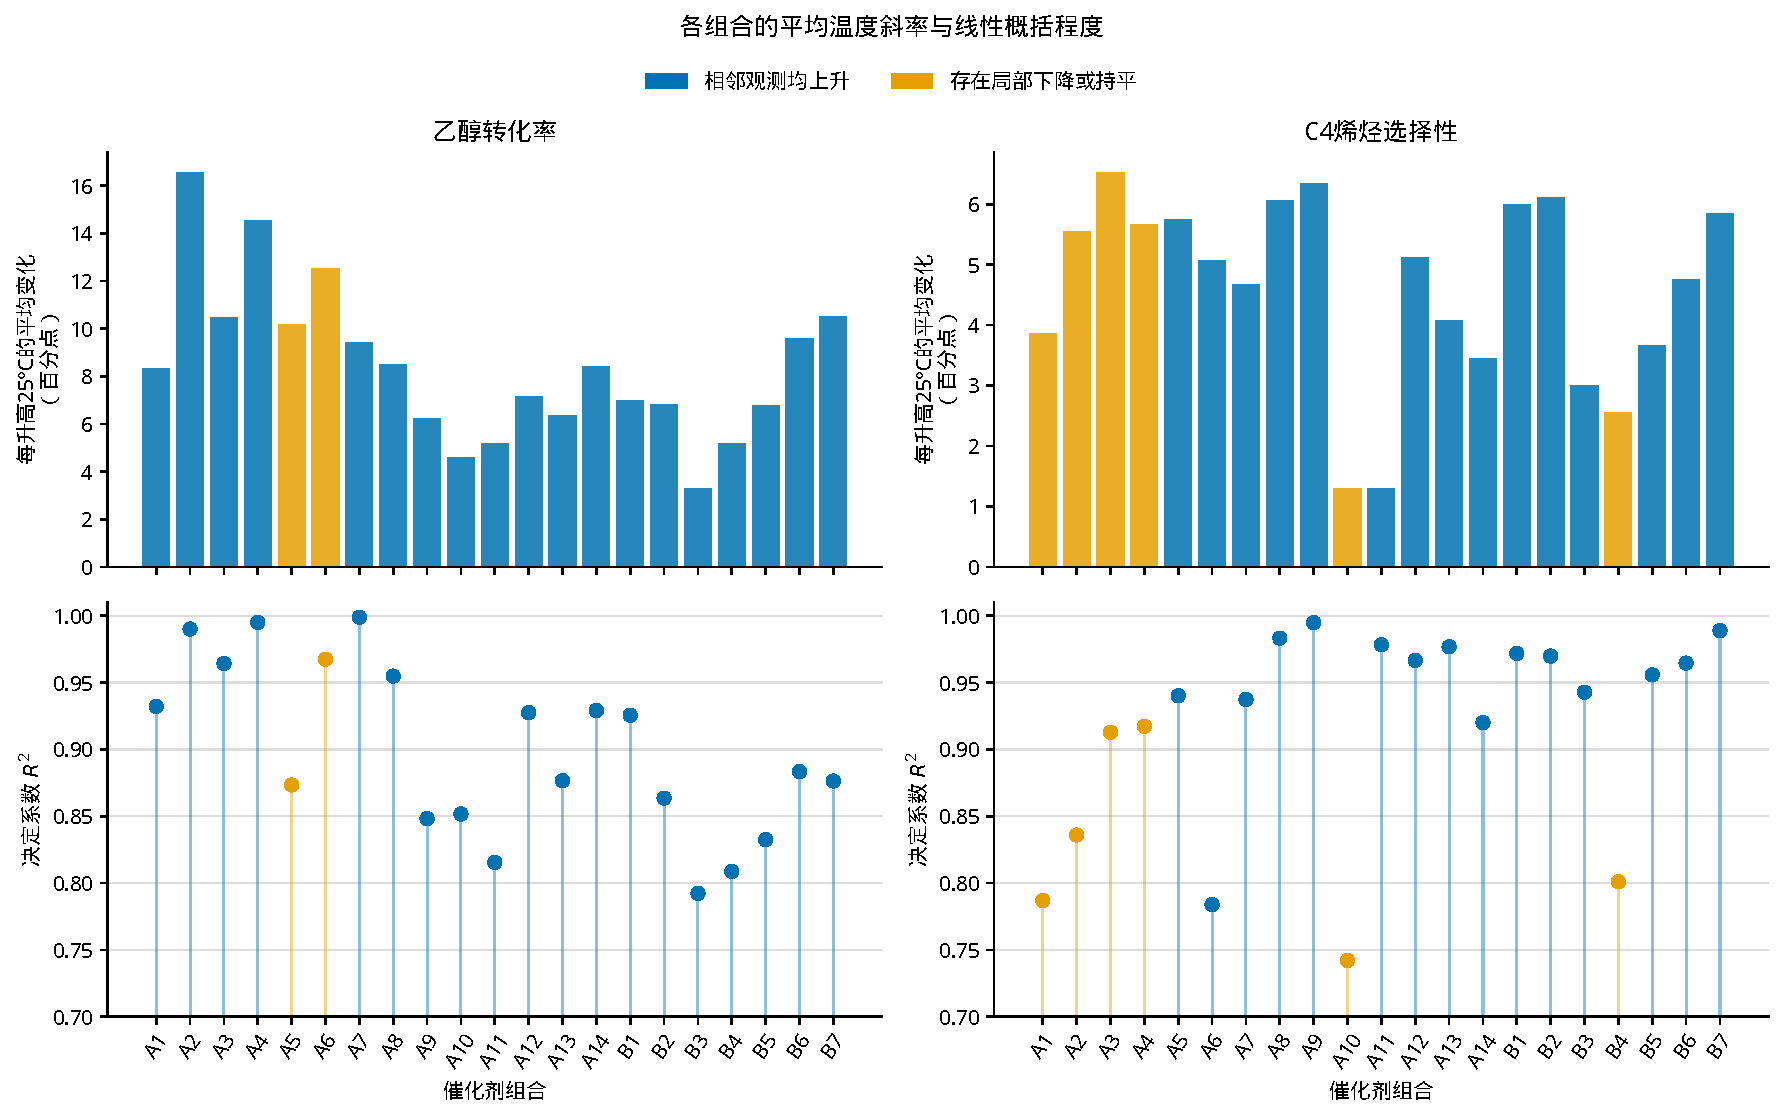
\includegraphics[width=\linewidth]{../../output/q1/figures/05_attachment1_linear_summary_diagnostics.pdf}
\caption{各催化剂组合在已测范围内的平均温度斜率与决定系数。上排分别给出乙醇转化率
和 C4 烯烃选择性每升高 25 ℃的平均变化量，下排给出对应 \(R^2\)。橙色表示该组合
至少存在一个局部下降或持平区间，蓝色表示全部相邻观测均上升。}
\label{fig:q1-linear-summary}
\end{figure}

该图显示，42条拟合直线的斜率均为正，但不同组合的斜率和
拟合程度差异明显。以A10为例，其选择性斜率为正，\(R^2=0.7421\)，但250---275 ℃
间实际下降，因此应描述为“平均正向，局部下降”。

综合42组结果，13种组合的两个指标在全部相邻温度下均升高；其余8种组合至少有一个
指标出现局部下降或持平。由此，第一问对各组合的回答统一为两类：“平均正向且无已测
局部例外”或“平均正向并伴随具体局部例外”。该结论限于各组合的已测温度范围。

\paragraph{附件 1 的计算一致性检验}

独立程序重新读取附件1，复算42组斜率、决定系数、相邻温度差和228次删点斜率，所得
结果与正文一致。该复算验证了计算过程，但现有数据仍不足以确定精确转折点或预测未测
温度。

\subsubsection{附件 2：一次实验的时间变化}

\paragraph{时间变化与稳定性判断}

设附件 2 时刻 t 的乙醇转化率、C4 烯烃选择性和收率分别为 X(t)、S(t) 和 Y(t)。
由于 7 个时刻间隔不等，所有变化速度均按真实分钟数计算。对总体下降方向清晰的转化率
和收率，建立只适用于 20---273 min 已观测区间的简单时间关系：

\begin{align}
X(t)&=\alpha_X+\beta_Xt+\varepsilon_X, \tag{10}\label{eq:q1-time-x}\\
Y(t)&=\alpha_Y+\beta_Yt+\varepsilon_Y. \tag{11}\label{eq:q1-time-y}
\end{align}

C4 烯烃选择性只在较窄范围内波动，因而用取值范围和首末变化描述；转化率和收率具有
清楚的下降趋势，因而再用式\eqref{eq:q1-time-x}和式\eqref{eq:q1-time-y}概括其平均变化速度。这里的``稳定''仅指
指标在本次观测时段内是否围绕近似固定水平小幅波动，不代表催化剂具有长期稳定性。

计算时，先由题给关系 \(Y(t)=X(t)S(t)/100\) 求出各时刻的 C4 烯烃收率。由于相邻观测
之间相隔 33---50 min，不能直接比较相邻差值，故将变化量统一换算为每 10 min 的变化：

\begin{align}
\Delta Z_j&=Z(t_{j+1})-Z(t_j),\notag\\
v_j&=\frac{10\Delta Z_j}{t_{j+1}-t_j}.
\tag{12}\label{eq:q1-time-change}
\end{align}

式\eqref{eq:q1-time-change}使不同长度的时间区间可以直接比较。再以真实时间 \(t\) 为自变量进行最小二乘
回归，并报告 \(10\beta\)，即每 10 min 的平均变化量。

7 个时刻的转化率由 43.5474\% 总体降至 29.9060\%，收率由 17.3754\% 总体降至
11.6753\%。两项指标均有清晰下降主线。C4 烯烃选择性则先降、后升、再波动，首末仅相差
0.86 个百分点。
因此，前两项用直线概括平均速度，选择性则保留实际范围和逐时刻变化。

\[
\widehat X(t)=42.6709-0.05276t,\qquad
\widehat Y(t)=16.5297-0.01989t .
\]

上述两式只概括 20---273 min 内的平均趋势。其中截距用于确定直线位置，不解释为
反应开始时刻的真实数值。

图\ref{fig:q1-time-regression}比较实际观测与20---273 min内的线性概括。
\begin{figure}[H]
\centering
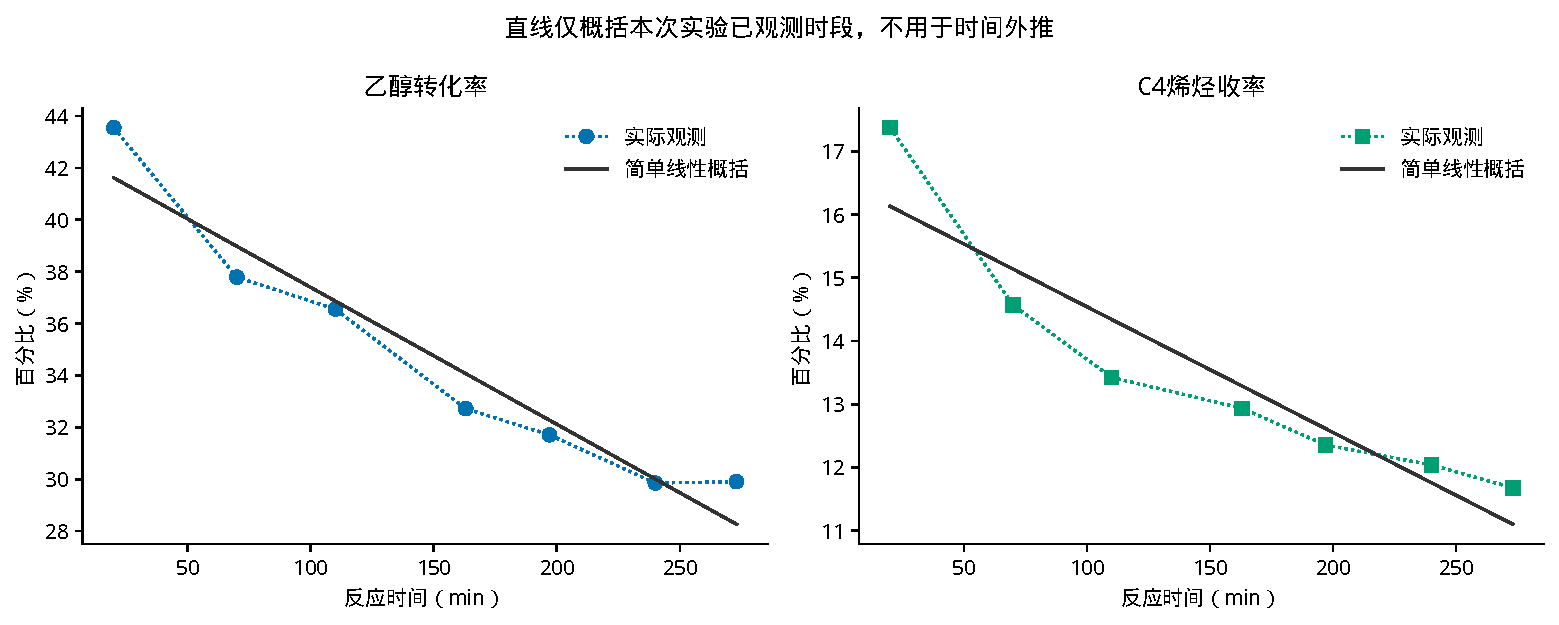
\includegraphics[width=0.90\linewidth]{../../output/q1/figures/06_attachment2_limited_linear_summaries.pdf}
\caption{附件 2 中乙醇转化率和 C4 烯烃收率的实际观测与线性概括。点线为实际观测，
黑色实线为 20---273 min 区间内的一元线性回归结果。}
\label{fig:q1-time-regression}
\end{figure}

由图可见，20---273 min 内乙醇转化率由 43.5474\% 降至 29.9060\%，下降
13.6414 个百分点；C4 烯烃收率由 17.3754\% 降至 11.6753\%，下降 5.7001 个百分点。
线性概括给出的平均速度分别为每 10 min 下降 0.5276 和 0.1989 个百分点，对应 $R^2$
分别为 0.9329 和 0.8575。实际点在前期下降较快、后期趋缓，且转化率在 240---273 min
回升 0.0518 个百分点，所以两条直线不能代替各时刻的真实变化。

C4 烯烃选择性由 39.90\% 变为 39.04\%，全过程位于 36.72\%---40.32\% 之间。与转化率和
收率的明显下降相比，选择性只在较小区间波动，表明本次实验中收率下降主要伴随乙醇
转化率降低，而不是由 C4 烯烃选择性持续下降造成。按上述判据，本次实验的选择性相对
稳定，但转化率和收率存在明显向下漂移，因而不能把整个反应表现概括为稳定。

\paragraph{产物份额的重新分配}

对每个时刻 t，六类产物选择性满足：

\begin{equation}
\sum_{k=1}^{6}P_k(t)=100\%.
\tag{13}\label{eq:q1-composition-sum}
\end{equation}

六类选择性合计为 100\%，所以它们表示产物组成中的相对份额。一类份额上升时，其他
类别的合计份额必然下降；这里研究的是产物组成如何变化，而不是六类产量各自如何变化。

除逐类比较首末份额外，再以C4 烯烃选择性为共同参照，定义：

\begin{align}
r_A(t)&=\frac{\text{乙醛选择性}}{\text{C4 烯烃选择性}},\notag\\
r_H(t)&=\frac{\text{C4---C12 脂肪醇选择性}}{\text{C4 烯烃选择性}}.
\tag{14}
\end{align}

\(r_A\) 和 \(r_H\) 分别比较乙醛、C4---C12 脂肪醇与 C4 烯烃的相对份额。前者增大
表示乙醛相对增多，后者减小表示脂肪醇相对减少；这两个比值不代表反应速率或直接转化。

图\ref{fig:q1-product-shares}同时展示六类产物份额和两项相对份额比的时间变化。
\begin{figure}[H]
\centering
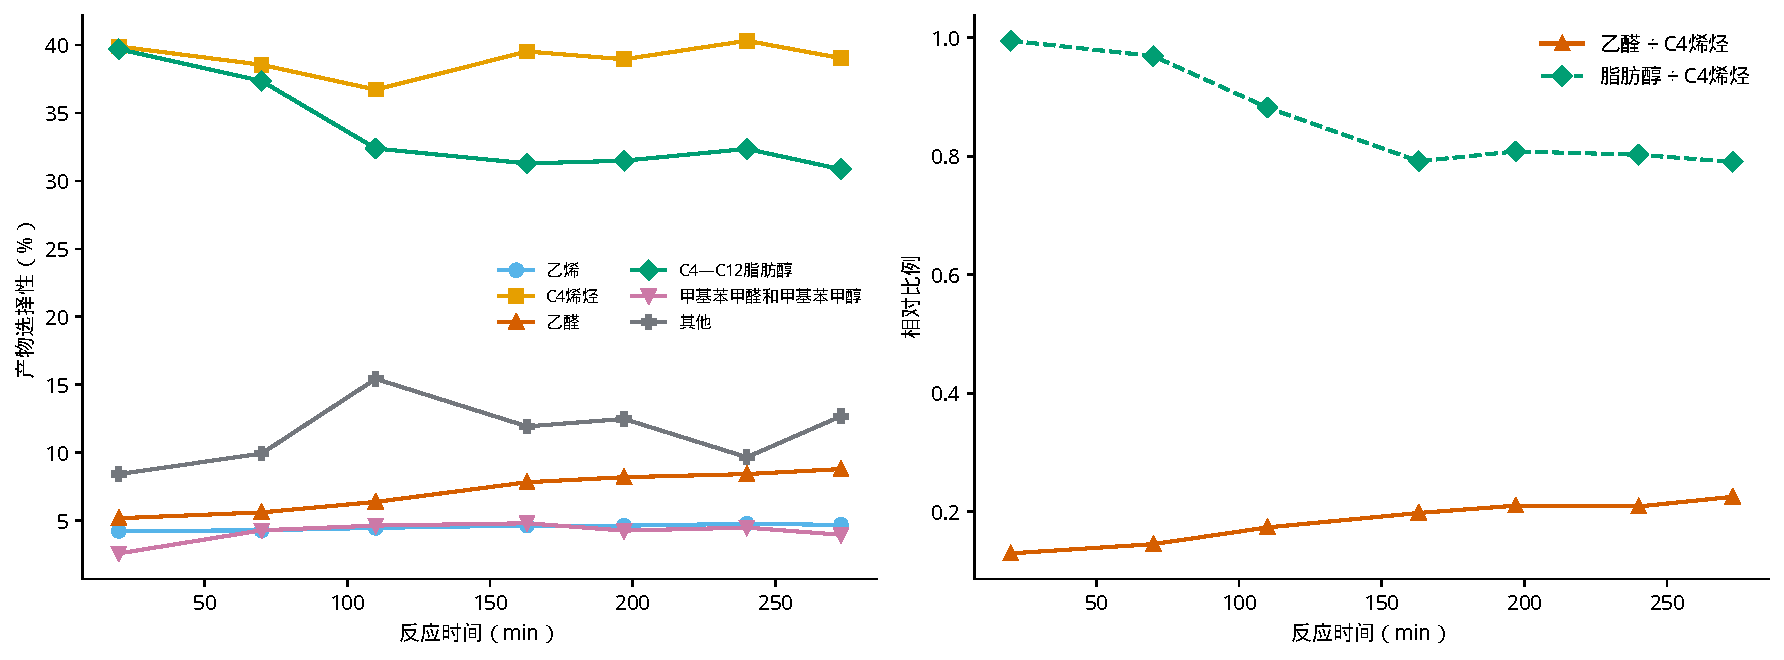
\includegraphics[width=0.90\linewidth]{../../output/q1/figures/03_attachment2_product_shares_and_ratios.pdf}
\caption{附件 2 中六类产物选择性及两项相对份额比随时间的变化。左图给出固定总和
份额的重新分配，右图给出乙醛和 C4---C12 脂肪醇相对 C4 烯烃的份额比。}
\label{fig:q1-product-shares}
\end{figure}

图中C4 烯烃选择性变化较小，但乙醛份额总体增加、
C4---C12 脂肪醇份额总体下降。为精确核对首末变化，表\ref{tab:q1-product-change}
列出 20 min 到 273 min 的百分点差。

\begin{table}[H]
\centering
\caption{附件 2 六类产物选择性的首末变化}
\label{tab:q1-product-change}
\begin{tabular}{lr}
\toprule\noalign{}
产物类别 & 首末变化/百分点 \\
\midrule\noalign{}
乙烯 & +0.45 \\
C4 烯烃 & −0.86 \\
乙醛 & +3.62 \\
C4---C12 脂肪醇 & −8.84 \\
甲基苯甲醛和甲基苯甲醇 & +1.37 \\
其他产物 & +4.26 \\
\bottomrule
\end{tabular}
\end{table}

增加项和减少项均合计 9.70 个百分点，与式\eqref{eq:q1-composition-sum}相符。
同期，乙醛与 C4 烯烃的份额比由 0.1296 升至 0.2252，C4---C12 脂肪醇与 C4 烯烃的
份额比由 0.9950 降至 0.7905。由此可见，即使 C4 烯烃选择性变化较小，产物内部结构
仍发生了明显调整，最突出的是脂肪醇份额下降而乙醛和其他产物份额上升。

已有研究表明，乙醛、较高碳数醇和烯烃可能处在相互衔接或竞争的反应路径中
\cite{ho2016,moteki2016,sushkevich2017}。这些研究为不同产物份额的同步变化提供了
可能的路径背景，但本题
缺少中间体示踪和反应速率数据，不能由此断言脂肪醇直接转化为 C4 烯烃。

\paragraph{测试现象的可能解释}

附件 2 中，乙醇转化率与 C4 烯烃收率同步下降，而 C4 烯烃选择性变化较小。这说明
目标产出降低主要来自乙醇转化率下降，而不是 C4 烯烃在产物中所占比例持续下降。若
催化剂的有效活性位在运行中减少或被覆盖，就可能出现这种``转化能力下降、主要产物
比例变化较小''的现象。

Yan 等在 Zn-Y/Beta 催化乙醇制丁二烯的实验中发现，含氧中间体继续缩合形成的物质会
逐渐覆盖活性位并导致催化剂失活 \cite{yan2018}。因此，活性位被覆盖可作为转化率下降
的一种可能解释。不过，该研究采用的催化剂和目标产物与本题不同，不能据此认定附件 2
中的催化剂发生了相同变化。

羟基磷灰石催化体系的研究还表明，乙醛可参与后续碳链增长，而生成较高碳数产物需要
继续经历缩合、氢转移和脱水等步骤 \cite{ho2016,moteki2016}。因此，若后续转化受到的
影响更强，乙醛的相对份额可能上升，较高碳数醇的份额可能下降。这与附件 2 的现象
相容，但选择性只是相对份额，不能据此判断乙醛的绝对生成量或证明产物之间直接转化。

时间序列还表现为前期下降较快、后期趋缓，最后一个区间轻微回升。这可能是体系逐渐
接近新的运行状态，也可能来自测量或操作波动。由于只有一次实验，且缺少催化剂表面
表征和重复测试，本文只把``活性位覆盖''和``后续转化受抑''列为可能机制，不作唯一
判断。

\paragraph{附件 2 的计算一致性检验}

独立程序复算了各时刻收率、时间斜率、两项份额比和六类选择性的首末变化，并确认每个
时刻六类份额合计为 100\%。复算结果与正文和图表一致。

\subsubsection{问题一结论与适用范围}

附件 1 的 21 种组合中，乙醇转化率和 C4 烯烃选择性的回归斜率均为正，且逐次删除一个
温度点后方向仍不改变，说明总体正向关系不依赖某个单点。但相邻观测显示，A5、A6 的
转化率以及 A1、A2、A3、A4、A10、B4 的选择性存在局部下降或持平。因此，温度与两项
指标在已测范围内总体呈正向关系，同时有 8 种组合存在局部例外。

对附件 2 的一次 350 ℃ 实验，20---273 min 内转化率和 C4 烯烃收率总体下降，每
10 min 的平均下降量分别为 0.5276 和 0.1989 个百分点；C4 烯烃选择性只在
36.72\%---40.32\% 之间波动。六类产物份额发生重新分配，其中 C4---C12 脂肪醇份额明显
下降，乙醛和其他产物份额总体增加。上述时间结论只适用于本次实验的已观测时段，不
推广为所有催化剂组合的一般规律。
